\pdfbookmark{Общая характеристика работы}{characteristic}             % Закладка pdf
\section*{Общая характеристика работы}

\newcommand{\actuality}{\pdfbookmark[1]{Актуальность}{actuality}\underline{\textbf{\actualityTXT}}}
\newcommand{\progress}{\pdfbookmark[1]{Разработанность темы}{progress}\underline{\textbf{\progressTXT}}}
\newcommand{\aim}{\pdfbookmark[1]{Цели}{aim}\underline{{\textbf\aimTXT}}}
\newcommand{\tasks}{\pdfbookmark[1]{Задачи}{tasks}\underline{\textbf{\tasksTXT}}}
\newcommand{\aimtasks}{\pdfbookmark[1]{Цели и задачи}{aimtasks}\aimtasksTXT}
\newcommand{\novelty}{\pdfbookmark[1]{Научная новизна}{novelty}\underline{\textbf{\noveltyTXT}}}
\newcommand{\influence}{\pdfbookmark[1]{Практическая значимость}{influence}\underline{\textbf{\influenceTXT}}}
\newcommand{\methods}{\pdfbookmark[1]{Методология и методы исследования}{methods}\underline{\textbf{\methodsTXT}}}
\newcommand{\defpositions}{\pdfbookmark[1]{Основные положения, выносимые на защиту}{defpositions}\underline{\textbf{\defpositionsTXT}}}
\newcommand{\reliability}{\pdfbookmark[1]{Достоверность}{reliability}\underline{\textbf{\reliabilityTXT}}}
\newcommand{\probation}{\pdfbookmark[1]{Апробация}{probation}\underline{\textbf{\probationTXT}}}
\newcommand{\contribution}{\pdfbookmark[1]{Личный вклад}{contribution}\underline{\textbf{\contributionTXT}}}
\newcommand{\publications}{\pdfbookmark[1]{Публикации}{publications}\underline{\textbf{\publicationsTXT}}}
\newcommand{\structureandsize}{\pdfbookmark[1]{Структура и объем работы}{structureandsize}\underline{\textbf{\structureandsizeTXT}}}


{\actuality} 

В настоящее время в разных областях биологии и медицины повсеместно используются цифровые изображения и развиваются алгоритмы их обработки, в том числе и на основе глубокого обучения. Несмотря на быстрый научно"=технический прогресс, в силу различных причин оборудование, используемое для получения таких изображений, не всегда способно решить возникающие задачи, однако применение математических методов позволяет приблизиться к их решению и повысить качество уже полученных данных. Поэтому разработка алгоритмов повышения качества изображений с учётом современных условий остаётся актуальной.

Изображения клеточных структур, возникающие в области флуоресцентной микроскопии, являются одним из классов изображений, увеличение разрешения которых необходимо на практике. Одними из примеров таких задач являются ситуации, при которых разрешающая способность оптической системы микроскопа упирается в теоретический предел из-за дифракции света или когда увеличение оптической системы микроскопа не позволяет реализовать весь потенциал теоретической разрешающей способности.

Хотя появились методики преодоления дифракционного предела с использованием специального оборудования, на практике более доступным подходом является использование специальных стохастический мигающих красителей. Серия снимков, на которых молекулы красителя имеют разную яркость, преобразуется в изображение повышенного разрешения. Благодаря повышенному по сравнению с одним снимком количеству информации и слабой корреляции мигания молекул флуорофора, вычислительные методы позволяют существенно повысить разрешающие способности микроскопов без дорогостоящей модификации оборудования. В то же время из-за необходимости получать большое число изображений за короткий срок, повышается значимость таких параметров, как уровень шума и скорость выгорания красителей.

Для макроскопических же изображений в медицине по причине строгих ограничений со стороны закона и специфики области, связанной с повышенными рисками ошибок, важен вопрос аккуратной обработки изображений для избежания потери или привнесения информации в имеющиеся данные и контроля качества получаемых изображений. Очень актуальна задача повышения резкости изображений. А для методов глубокого обучения в медицинской диагностике, которые внедряются в практику во всём мире, является анализ и предобработка входных данных. Необходим контроль соответствия входной информации и применяемого обученного или обучаемого алгоритма глубокого обучения.

При изучении рентгеновских снимков и, в частности, при диагностике туберкулёза лёгких важным фактором является жёсткость снимка, так как она напрямую влияет на его информативность: на изображении должны в достаточном количестве присутствовать важные для вынесения верного решения детали. Кроме того, необходима правильная настройка контрастности снимков, чтобы различия изображений из обучающего набора и тестовых снимков, которые получаются на различном оборудовании в разных условиях, не были велики настолько, чтобы влиять на качество работы алгоритмов диагностики.

Основное внимание в данной работе уделено повышению качества изображений клеточных структур и анализу качества медицинских изображений. Под качеством понимается как наличие у изображения определённых характеристик (резкость, контрастность, разрешение), так и их степень сходства с эталонными изображениями, для работы с которыми оптимизирован алгоритм машинного или глубокого обучения.

%\ifsynopsis
%Этот абзац появляется только в~автореферате.
%Для формирования блоков, которые будут обрабатываться только в~автореферате,
%заведена проверка условия \verb!\!\verb!ifsynopsis!.
%Значение условия задаётся в~основном файле документа (\verb!synopsis.tex! для
%автореферата).
%\else
%Этот абзац появляется только в~диссертации.
%Через проверку условия \verb!\!\verb!ifsynopsis!, задаваемого в~основном файле
%документа (\verb!dissertation.tex! для диссертации), можно сделать новую
%команду, обеспечивающую появление цитаты в~диссертации, но~не~в~автореферате.
%\fi

% {\progress}
% Этот раздел должен быть отдельным структурным элементом по
% ГОСТ, но он, как правило, включается в описание актуальности
% темы. Нужен он отдельным структурынм элемементом или нет ---
% смотрите другие диссертации вашего совета, скорее всего не нужен.


{\aim}

Цель данной работы состоит в разработке адаптивных методов анализа и обработки биомедицинских изображений различных модальностей на основе методов \fixme{математического моделирования}, их алгоритмическая и программная реализация для решения задач повышения разрешения изображений флуоресцентной микроскопии, повышения резкости и контроля качества медицинских изображений.


{\novelty}

В данной работе были получены новые методы и алгоритмы:
\begin{enumerate}[beginpenalty=10000]
	\item \fixme{регуляризирующий метод повышения разрешения и резкости изображений флуоресцентной мигающей микроскопии;}
	
	\item \fixme{малопараметрический деформационный метод повышения резкости изображений;}
	
	\item \fixme{нейросетевой метод контроля качества рентгеновских снимков грудной клетки, основанный на автоматическом анализе жёсткости рентгенограммы;}
	
	\item \fixme{алгоритм компьютерной диагностики туберкулёза лёгких по рентгеновскому снимку грудной клетки.}
\end{enumerate}


{\influence}

Создан программный комплекс повышения разрешения изображений флуоресцентной мигающей микроскопии, повышения резкости медицинских изображений и определения качества рентгенограмм грудной клетки для задачи диагностики туберкулёза лёгких.

Предложенные методы могут применяться как отдельно, так и в составе других систем анализа и повышения качества биомедицинских изображений, в качестве вспомогательных инструментов в работе учёных-биологов и врачей, а также могут быть модифицированы для применения в иных областях медицины и биологии, отличных от рассмотренных в работе.


{\progress}

Исследование, проведённое в данной работе, затрагивает три различных области анализа и повышения качества биомедицинских изображений.

В области флуоресцентной микроскопии, получившей распространение благодаря таким своим достоинствам, как высокий контраст получаемых изображений, возможность избирательного окрашивания структур разной природы в разные цвета и наблюдения за живыми образцами, к настоящему времени был разработан ряд методов повышения разрешающей способности микроскопов. Некоторые из них (конфокальная микроскопия, STED, SIM) требуют особого оборудования, другие же (STORM, PALM, SOFI, SRRF, MUSICAL) появились уже в 21 веке и полагаются на использование специальных мигающих красителей и вычислительные алгоритмы.

В прошлом и в текущем веке было разработано множество эффективных методов повышения резкости и восстановления смазанных изображений. Многие из них требуют указания типа размытия для работы, и хотя за последние 20 лет появились алгоритмы автоматического определения размытия по входному изображению, чувствительность методов повышения резкости к шуму и ошибкам в определении и указании типа и силы размытия остаётся значимым фактором. Метод повышения резкости изображений с помощью деформации пиксельной сетки не предназначен для решения задачи полноценного восстановления смазанных изображений, но может служить в качестве этапа постобработки восстановленного другим алгоритмом изображения, повышая резкость без порождения артефактов на изображении. Выбор оптимальной функции смещения пикселей позволяет регулировать эффективность обработки изображения.

С новым витком развития области науки в середине 2010"~х годов и повсеместном распространении алгоритмов на основе искусственного интеллекта и глубокого обучения вопрос о влиянии качества входных данных на результаты обработки и о контроле качества этих данных снова получил высокую актуальность. За последнее десятилетие были проведены исследования на тему целенаправленных атак на алгоритмы анализа данных с целью повлиять на результаты их работы путём незаметного для человека изменения входных данных и защиты от таких атак. В то же время в области медицинской диагностики заболеваний по рентгенограммам грудной клетки за последние 10 лет были разработаны методы контроля некоторых условий съёмки, изучено влияние качества снимков на точность диагностики некоторых заболеваний.


{\methods} 

В основе методологии исследования лежат \fixme{методы математического моделирования} в обработке и анализе изображений, ряд вычислительных экспериментов реализован в рамках задач машинного обучения и анализа изображений с помощью искусственных и реальных данных.


{\reliability}

Достоверность результатов проведённых исследований обеспечивается опорой на теоретическую базу, математической обоснованностью разработанных методов, воспроизводимыми вычислительными экспериментами и тестированием алгоритмов на искусственных и реальных данных. Значительная часть данных, использованных для создания и тестирования разработанных методов, находится в открытом доступе.


{\probation}
Основные результаты работы докладывались на:

\begin {enumerate}[beginpenalty=10000]
	\item 7-й Международной конференции по теории обработки изображений, методам и применениям <<IPTA 2017>> (Монреаль, Канада, 2017);
	
	\item 7-м Европейском семинаре по обработке визуальной информации <<EUVIP~2018>> (Тампере, Финляндия, 2018);
	
	\item 4"~й Международной конференции по обработке биомедицинских изображений и сигналов <<ICBSP~2019>> (Нагоя, Япония, 2019);
	
	\item Всероссийской конференции <<Ломоносовские чтения"~2020>> (Москва, 2020);
	
	\item 6"~й Международной конференции по обработке биомедицинских изображений и сигналов <<ICBSP~2021>> (Сямынь, Китай, 2021);
\end {enumerate}

\ifnumequal{\value{bibliosel}}{0}
{%%% Встроенная реализация с загрузкой файла через движок bibtex8. (При желании, внутри можно использовать обычные ссылки, наподобие `\cite{vakbib1,vakbib2}`).
    {\publications}
    
    По теме исследования опубликовано~8~работ, из них~6~работ в изданиях, идексируемых системами \fixme{Scopus, Web of Science, RSCI, а также в изданиях, рекомендуемых для защиты в диссертационном совете МГУ имени М.В.~Ломоносова} по специальности 1.2.2.~<<Математическое моделирование, численные методы и комплексы программ>>, и~2~работы, опубликованные в иных изданиях.
    
%    Основные результаты по теме диссертации изложены
%    в~XX~печатных изданиях,
%    X из которых изданы в журналах, рекомендованных ВАК,
%    X "--- в тезисах докладов.
}%
{%%% Реализация пакетом biblatex через движок biber
    \begin{refsection}[bl-author, bl-registered]
        % Это refsection=1.
        % Процитированные здесь работы:
        %  * подсчитываются, для автоматического составления фразы "Основные результаты ..."
        %  * попадают в авторскую библиографию, при usefootcite==0 и стиле `\insertbiblioauthor` или `\insertbiblioauthorgrouped`
        %  * нумеруются там в зависимости от порядка команд `\printbibliography` в этом разделе.
        %  * при использовании `\insertbiblioauthorgrouped`, порядок команд `\printbibliography` в нём должен быть тем же (см. biblio/biblatex.tex)
        %
        % Невидимый библиографический список для подсчёта количества публикаций:
        \printbibliography[heading=nobibheading, section=1, env=countauthorvak,          keyword=biblioauthorvak]%
        \printbibliography[heading=nobibheading, section=1, env=countauthorwos,          keyword=biblioauthorwos]%
        \printbibliography[heading=nobibheading, section=1, env=countauthorscopus,       keyword=biblioauthorscopus]%
        \printbibliography[heading=nobibheading, section=1, env=countauthorconf,         keyword=biblioauthorconf]%
        \printbibliography[heading=nobibheading, section=1, env=countauthorother,        keyword=biblioauthorother]%
        \printbibliography[heading=nobibheading, section=1, env=countregistered,         keyword=biblioregistered]%
        \printbibliography[heading=nobibheading, section=1, env=countauthorpatent,       keyword=biblioauthorpatent]%
        \printbibliography[heading=nobibheading, section=1, env=countauthorprogram,      keyword=biblioauthorprogram]%
        \printbibliography[heading=nobibheading, section=1, env=countauthor,             keyword=biblioauthor]%
        \printbibliography[heading=nobibheading, section=1, env=countauthorvakscopuswos, filter=vakscopuswos]%
        \printbibliography[heading=nobibheading, section=1, env=countauthorscopuswos,    filter=scopuswos]%
        %
        \nocite{*}%
        %
        {\publications}
        
        По теме исследования опубликовано~8~работ, из них~6~работ в изданиях, идексируемых системами \fixme{Scopus, Web of Science, RSCI, а также в изданиях, рекомендуемых для защиты в диссертационном совете МГУ имени М.В.~Ломоносова} по специальности 1.2.2.~<<Математическое моделирование, численные методы и комплексы программ>>, и~2~работы, опубликованные в иных изданиях.
        
%        Основные результаты по теме диссертации изложены в~\arabic{citeauthor}~печатных изданиях,
%        \arabic{citeauthorvak} из которых изданы в журналах, рекомендованных ВАК\sloppy%
%        \ifnum \value{citeauthorscopuswos}>0%
%            , \arabic{citeauthorscopuswos} "--- в~периодических научных журналах, индексируемых Web of~Science и Scopus\sloppy%
%        \fi%
%        \ifnum \value{citeauthorconf}>0%
%            , \arabic{citeauthorconf} "--- в~тезисах докладов.
%        \else%
%            .
%        \fi%
%        \ifnum \value{citeregistered}=1%
%            \ifnum \value{citeauthorpatent}=1%
%                Зарегистрирован \arabic{citeauthorpatent} патент.
%            \fi%
%            \ifnum \value{citeauthorprogram}=1%
%                Зарегистрирована \arabic{citeauthorprogram} программа для ЭВМ.
%            \fi%
%        \fi%
%        \ifnum \value{citeregistered}>1%
%            Зарегистрированы\ %
%            \ifnum \value{citeauthorpatent}>0%
%            \formbytotal{citeauthorpatent}{патент}{}{а}{}\sloppy%
%            \ifnum \value{citeauthorprogram}=0 . \else \ и~\fi%
%            \fi%
%            \ifnum \value{citeauthorprogram}>0%
%            \formbytotal{citeauthorprogram}{программ}{а}{ы}{} для ЭВМ.
%            \fi%
%        \fi%
        % К публикациям, в которых излагаются основные научные результаты диссертации на соискание учёной
        % степени, в рецензируемых изданиях приравниваются патенты на изобретения, патенты (свидетельства) на
        % полезную модель, патенты на промышленный образец, патенты на селекционные достижения, свидетельства
        % на программу для электронных вычислительных машин, базу данных, топологию интегральных микросхем,
        % зарегистрированные в установленном порядке.(в ред. Постановления Правительства РФ от 21.04.2016 N 335)
    \end{refsection}%
    \begin{refsection}[bl-author, bl-registered]
        % Это refsection=2.
        % Процитированные здесь работы:
        %  * попадают в авторскую библиографию, при usefootcite==0 и стиле `\insertbiblioauthorimportant`.
        %  * ни на что не влияют в противном случае
%        \nocite{vakbib2}%vak
%        \nocite{patbib1}%patent
%        \nocite{progbib1}%program
%        \nocite{bib1}%other
%        \nocite{confbib1}%conf
    \end{refsection}%
        %
        % Всё, что вне этих двух refsection, это refsection=0,
        %  * для диссертации - это нормальные ссылки, попадающие в обычную библиографию
        %  * для автореферата:
        %     * при usefootcite==0, ссылка корректно сработает только для источника из `external.bib`. Для своих работ --- напечатает "[0]" (и даже Warning не вылезет).
        %     * при usefootcite==1, ссылка сработает нормально. В авторской библиографии будут только процитированные в refsection=0 работы.
}

%При использовании пакета \verb!biblatex! будут подсчитаны все работы, добавленные
%в файл \verb!biblio/author.bib!. Для правильного подсчёта работ в~различных
%системах цитирования требуется использовать поля:
%\begin{itemize}
%        \item \texttt{authorvak} если публикация индексирована ВАК,
%        \item \texttt{authorscopus} если публикация индексирована Scopus,
%        \item \texttt{authorwos} если публикация индексирована Web of Science,
%        \item \texttt{authorconf} для докладов конференций,
%        \item \texttt{authorpatent} для патентов,
%        \item \texttt{authorprogram} для зарегистрированных программ для ЭВМ,
%        \item \texttt{authorother} для других публикаций.
%\end{itemize}
%Для подсчёта используются счётчики:
%\begin{itemize}
%        \item \texttt{citeauthorvak} для работ, индексируемых ВАК,
%        \item \texttt{citeauthorscopus} для работ, индексируемых Scopus,
%        \item \texttt{citeauthorwos} для работ, индексируемых Web of Science,
%        \item \texttt{citeauthorvakscopuswos} для работ, индексируемых одной из трёх баз,
%        \item \texttt{citeauthorscopuswos} для работ, индексируемых Scopus или Web of~Science,
%        \item \texttt{citeauthorconf} для докладов на конференциях,
%        \item \texttt{citeauthorother} для остальных работ,
%        \item \texttt{citeauthorpatent} для патентов,
%        \item \texttt{citeauthorprogram} для зарегистрированных программ для ЭВМ,
%        \item \texttt{citeauthor} для суммарного количества работ.
%\end{itemize}
%% Счётчик \texttt{citeexternal} используется для подсчёта процитированных публикаций;
%% \texttt{citeregistered} "--- для подсчёта суммарного количества патентов и программ для ЭВМ.
%
%Для добавления в список публикаций автора работ, которые не были процитированы в
%автореферате, требуется их~перечислить с использованием команды \verb!\nocite! в
%\verb!Synopsis/content.tex!.


{\contribution} 

Все результаты работы получены автором лично под научным руководством д.ф.-м.н., проф. А.С. Крылова. В работах, написанных в соавторстве, вклад автора работы в полученные результаты \fixme{математического моделирования, численные методы и разработку комплекса программ} является определяющим.


{\defpositions}

\begin {enumerate}[beginpenalty=10000]
	\item Итерационный регуляризирующий метод повышения разрешения изображений мигающей флуоресцентной микроскопии.
	
	\item Метод повышения резкости медицинских изображений на основе деформации пиксельной сетки для различных \fixme{математических моделей} оптического размытия изображений.
	
	\item Метод автоматического анализа качества рентгенограмм грудной клетки, основанный на нейросетевой оценке уровня жёсткости рентгеновских снимков.
	
	\item Программный комплекс, включающий модули повышения резкости медицинских изображений, повышения разрешения изображений мигающей флуоресцентной микроскопии и оценки уровня жёсткости рентгенограмм грудной клетки для задачи диагностики туберкулёза лёгких.
\end {enumerate}
 % Характеристика работы по структуре во введении и в автореферате не отличается (ГОСТ Р 7.0.11, пункты 5.3.1 и 9.2.1), потому её загружаем из одного и того же внешнего файла, предварительно задав форму выделения некоторым параметрам

%Диссертационная работа была выполнена при поддержке грантов \dots

\underline{\textbf{Структура и объем работы}}

Диссертация состоит из~введения, четырёх глав, заключения, списков литературы, публикаций автора по теме исследования, рисунков и таблиц. Полный объем диссертации составляет 104~страницы, включая 47~рисунков и~9~таблиц. Список литературы содержит 94~наименования.

\pdfbookmark{Содержание работы}{description}                          % Закладка pdf
\section*{Содержание работы}

%TODO Введение
Во {\textbf{введении}} обосновывается актуальность работы, изложены её цель, научная новизна и практическая ценность, даны основные характеристики работы, сформулированы положения, выносимые на защиту, личный вклад автора, представлен отчёт об апробации работы и публикациях, содержащих основные результаты.


%TODO Глава 1
В {\textbf{первой}} главе рассматривается проблема повышения разрешения и резкости изображений флуоресцентной микроскопии на основе анализа временной серии снимков образца, подсвеченного стохастически мигающим красителем (пример снимков такой серии приведён на Рис.~\ref{fig:sinopsis-blinking-samples}). Этот подход не требует специального оборудования для получения изображений повышенного разрешения, поэтому в настоящее время получил широкое распространение и продолжает активно развиваться. Для решения задачи построения резкого изображения высокого разрешения на основе последовательности изображений объекта, подсвеченного стохастически мигающим красителем, предложена математическая модель и разработан численный метод.

\begin{figure}[ht]
	\centerfloat{
		\hfill
		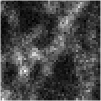
\includegraphics[width=0.18\textwidth]{blinking-1-6a.png}
		\hfill
		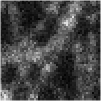
\includegraphics[width=0.18\textwidth]{blinking-1-6b.png}
		\hfill
		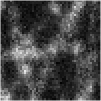
\includegraphics[width=0.18\textwidth]{blinking-1-6c.png}
		\hfill
		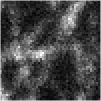
\includegraphics[width=0.18\textwidth]{blinking-1-6d.png}
		\hfill
		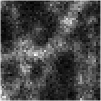
\includegraphics[width=0.18\textwidth]{blinking-1-6e.png}
		\hfill
	}
	\caption{Пример серии изображений, полученных с использованием мигающих флуорофоров}
	\label{fig:sinopsis-blinking-samples}
\end{figure}

Используемая модель искажения изображения флуоресцентной микроскопии имеет вид:

\begin{equation*}
	y_{ij} = \left(Kx+n\right)_{ij},\quad K=DB,
\end{equation*}

\noindent где $x$ "--- исходное резкое изображение высокого разрешения, $y$ "--- наблюдаемое изображение, $K$ "--- оператор размытия и понижения разрешения, действие которого эквивалентно последовательному действию оператора размытия $B$ и оператора понижения разрешения $D$ (производящего, например, усреднение групп соседних пикселей или простое прореживание пиксельной сетки изображения), а $n$ "--- аддитивный шум с нормальным распределением.

Рассматриваемая модель размытия изображения имеет вид свёртки изображения с ядром размытия:

\begin{equation*}
	x^\prime_{i,j} = \left(B \ast x\right)_{i,j} = \sum_{k=-\infty}^{\infty} \sum_{p=-\infty}^{\infty}{B_{k,p}\ x_{i-k,j-p}},
\end{equation*}

\noindent где $x$ "--- исходное резкое изображение, $x^\prime$ "--- искажённое изображение, $B$ "--- ядро размытия (англ.~point spread function, PSF).

Получившие широкое распространение конфокальные лазерные микроскопы позволяют, сканируя образец лазерным лучом, возбуждать молекулы флуорофора в малых областях образца и получать в итоге более чёткое изображение, чем  при подсветке всего образца сразу. Кроме того, флуоресцентное излучение со смежных слоёв образца, находящихся не в фокусе объектива, частично отсекается точечной диафрагмой, расположенной перед приёмником света. Базовая схема такого микроскопа представлена на Рис.~\ref{fig:sinopsis-scanning-microscope-scheme}.

\begin{figure}[ht]
	\centerfloat{
		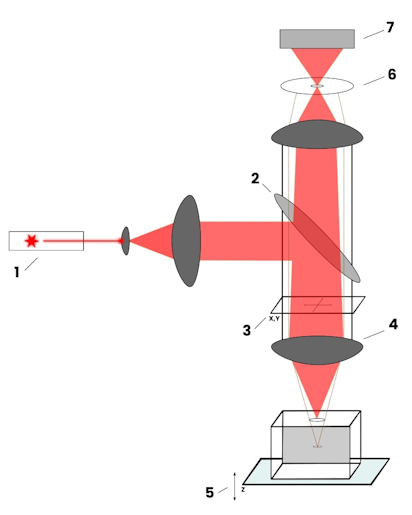
\includegraphics[height=0.4\textheight]{scanning-microscope-scheme.png}
	}
	\caption{Базовая схема конфокального лазерного сканирующего микроскопа. 1 "--- источник лазерного излучения; 2 "--- дихроичное зеркало, отражающее излучение с определённой длиной волны; 3 "--- механизм управления направлением луча лазера; 4 "--- линза объектива; 5 "--- механизм управления расстоянием от объектива до образца; 6 "--- точечная диафрагма; 7 "--- детектор флуоресцентного излучения.}
	\label{fig:sinopsis-scanning-microscope-scheme}
\end{figure}

Благодаря поточечной подсветке, ядро размытия в лазерном сканирующем микроскопе $PSF_{eff}$ определяется произведением ядра размытия лазерного луча подсветки образца $PSF_{exc}$ и ядра размытия объектива $PSF_{em}$.
% (см.~\cite{weisshart2014basic}). 
Каждое из этих ядер симметрично и задаётся формулами:

\begin{align*}
	&PSF\left(r, r_0\right) = I_0 \cdot \left(\frac{2\cdot J_1\left(v\right)}{v}\right)^2, \\
	&v=\frac{2\cdot\pi\cdot A\cdot\left|r-r_0\right|}{\lambda}, \\
	&J_1(v)=\sum_{n=0}^{\infty}{\left(-1\right)^n\frac{x^{2n+1}}{2^{2n+1}n!\left(n+1\right)!}},
\end{align*}

\noindent где $I_0$ "--- нормирующий множитель, $J_1$ "--- функция Бесселя первого рода первого порядка, $A$ "--- числовая апертура фокусирующей линзы, $r$ "--- точка в плоскости изображения, $r_0$ "--- центр ядра размытия в плоскости изображения, $\lambda$ "--- длина волны лазера подсветки или флуоресцентного излучения.

Итоговое ядро размытия получаемого микроскопом изображения имеет вид $PSF_{eff}\left(r\right)=PSF_{exc}\left(r,r_{0,exc}\right)\cdot PSF_{em}\left(r,r_{0,em}\right)$, где $r$ "--- точка на изображении, $r_{0,exc}$, $r_{0,em}$ "--- центры ядер размытия лазера подсветки и флуоресцентного излучения соответственно (см.~Рис.~\ref{fig:sinopsis-blinking-psf}).

\begin{figure}[ht]
	\centerfloat{
		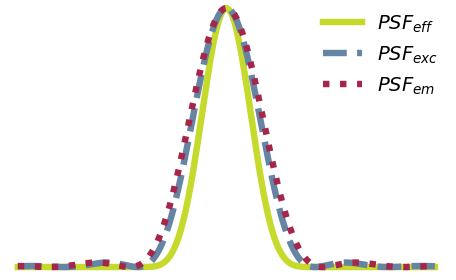
\includegraphics[height=0.2\textheight]{blinking-1-1-gray.png}
	}
	\caption{Нормированные профили ядер размытия лазера подсветки ($PSF_{exc}$), объектива ($PSF_{em}$) и микроскопа ($PSF_{eff}$)}
	\label{fig:sinopsis-blinking-psf}
\end{figure}

%В основе разработанного метода лежит предположение о том, что интенсивности пикселей резкого изображения можно рассмотреть как независимые случайные величины, а серию резких изображений "--- как результат серии наблюдений этих случайных величин. Влияние дифракции представлено свёрткой резкого изображения с одним и тем же ядром для всех пикселей и всех кадров, а полученные размытые снимки содержат высокочастотный шум.

На вход разработанного в данной работе алгоритма поступает набор размытых и зашумлённых изображений $Y=\left\{y^t\right\}_{t=1}^T$, $y^t\in\mathbb{R}^l$, ему соответствует неизвестный набор резких изображений высокого разрешения $X=\left\{x^t\right\}_{t=1}^T$, $x^t\in\mathbb{R}^n$. Благодаря природе шума, его можно моделировать случайным процессом с нормальным распределением.
%~\cite{gadsden1965some}. 
Поэтому в данном пункте считается, что $y^t \sim N({Kx}^t,\Theta^{-1})$, где $K\in\mathbb{R}^{l \times n}$ "--- оператор свёртки и понижения разрешения (имеет вид матрицы Тёплица с элементами ядра размытия на диагоналях, умноженной на матрицу понижения разрешения слева), а $\Theta\in\mathbb{R}^{n \times n}$ "--- обратная ковариационная матрица шума, диагональная из-за попиксельной независимости шума. Предполагается, что вследствие малого размера молекул флуорофора в каждом пикселе изображения может находиться достаточно много независимо мигающих молекул, чтобы можно было приблизить распределение суммарной яркости точки нормальным распределением: $x^t \sim N(\mu,\Lambda^{-1})$, где $\mu\in\mathbb{R}^n$ "--- средняя по всем кадрам яркость объекта, а $\Lambda\in\mathbb{R}^{n \times n}$ "--- обратная ковариационная матрица мерцания объекта.

Финальным результатом работы алгоритма являются оценки средней яркости образца $\mu$ и диагонали ковариационной матрицы $\Lambda^{-1}$, квадратные корни элементов которой является стандартными отклонениями яркостей точек резких изображений.

Для нахождения апостериорных распределений $\mu$ и $\Lambda$ и матрицы $\Theta$ максимизируется правдоподобие набора кадров $Y$ с помощью аппроксимации среднего поля и EM"~алгоритма: $p\left(Y\middle|\Theta\right) \rightarrow \max_{\Theta}$.
Необходимая для этого совместная плотность распределения $p\left(X,\mu,\Lambda\middle|Y,\Theta\right)$ определяется произведением:

$p\left(X,\mu,\Lambda\middle|Y,\Theta\right)=\frac{p\left(Y\middle|X,\Theta\right)p\left(X\middle|\mu,\Lambda\right)p\left(\mu\right)p\left(\Lambda\right)}{p\left(Y\middle|\Theta\right)}$.

Априорные распределения $p\left(\mu\right)$ и $p\left(\Lambda\right)$ в рамках исследования задаются следующим образом:

\begin{align*}
	&\mu \sim N\left(m_0,\ \eta_0^{-1}I_n\right), \\
	&\Lambda \sim W\left(W_0,\nu_0\right)=\frac{1}{C}\left|\Lambda\right|^\frac{\nu_0-n-1}{2}\exp{\left(-\frac{1}{2}tr\left[W_0^{-1}\Lambda\right]\right)},
\end{align*}

\noindent где $W(\cdots)$ "--- распределение Уишарта, $I_n$ "--- единичная матрица, $m_0\in\mathbb{R}^n$, $\eta_0,\ \nu_0\in\mathbb{R}$ и $W_0\in\mathbb{R}^{n \times n}$ "--- параметры метода, а $C$ "--- нормировочная константа.

Апостериорные распределения $\left\{x^t\right\}_{t=1}^T$, $\mu$ и $\Lambda$ аппроксимируются с помощью нормальных распределений $q_{1,t}\left(x^t\right)$ и $q_2\left(\mu\right)$ и распределения Уишарта $q_3\left(\Lambda\right)$, а плотностью вероятности их апостериорного совместного распределения аппроксимируется их произведением:

\begin{equation*}
	p\left(X,\mu,\Lambda\middle|Y,\Theta\right)\approx q\left(X,\mu,\Lambda\right)=\prod_{t=1}^{T}{q_{1,t}\left(x^t\right)\cdot\ q_2\left(\mu\right)\cdot q_3\left(\Lambda\right)}.
\end{equation*}

Итоговый алгоритм выглядит следующим образом:

\begin{enumerate}[beginpenalty=10000]
	\item Задаются начальные приближения некоторых параметров искомых распределений $\mu$ и $\Lambda$ и матрицу $\Theta$: $\mathbb{E}\mu \gets \mathbb{E}y^t$, $\mathbb{E}\Lambda \gets diag\left(D\left( y^t \right)\right)$, $\Theta \gets \theta I_l$, где $\theta$ "--- эмпирическая оценка шума, выполненная в пустой области изображения.
	
	\item В течение $R$ итераций происходит обновление параметров искомых распределений:
	
	\begin{align*}
		&q_{1,t}\left(x^t\right):\ \Sigma_{x^t} \gets \left(K^\mathrm{T} \Theta K+\mathbb{E}\Lambda\right)^{-1},\ \ \mathbb{E}x^t \gets \Sigma_{x^t} \cdot \left(K^\mathrm{T} \Theta y^t+\mathbb{E}\Lambda\cdot\mathbb{E}\mu\right); \\
		&q_2\left(\mu\right):\ \Sigma_\mu \gets \left(T\cdot\mathbb{E}\Lambda+\eta_0 I_n\right)^{-1},\ \ \mathbb{E}\mu \gets \Sigma_\mu \cdot \left(\mathbb{E}\Lambda\cdot\sum_{t=1}^{T}{\mathbb{E}x^t}+\eta_0 I_nm_0\right); \\
		&q_3\left(\Lambda\right):\ W\left(W^\prime,v^\prime\right),\ v^\prime \gets v_0+T, \\
		&W^\prime \gets \left(W_0^{-1}+\sum_{t=1}^{T}\left[
		\begin{aligned}
			&\Sigma_{x^t} + \mathbb{E}x^t\left(\mathbb{E}x^t\right)^\mathrm{T} - \mathbb{E}x^t\left(\mathbb{E}\mu\right)^\mathrm{T} - \\
			&- \mathbb{E}\mu\left(\mathbb{E}x^t\right)^\mathrm{T} + \Sigma_\mu + \mathbb{E}\mu\left(\mathbb{E}\mu\right)^\mathrm{T}
		\end{aligned}
		\right]\right)^{-1}, \\
		&\mathbb{E}\Lambda \gets v^\prime W^\prime; \\
		%	&\Theta \gets \left(\frac{1}{T}\sum_{t=1}^{T}\left[\left(K\mathbb{E}x^t-y^t\right)\left(K\mathbb{E}x^t-y^t\right)^\mathrm{T}+K\Sigma_{x^t}K^\mathrm{T}\right]\right)^{-1}. \\
		&\Theta_{ii} \gets \left(\frac{1}{T}\sum_{t=1}^{T}\left[\left(\left(K\mathbb{E}x^t - y^t\right)_i\right)^2 + \left(K\Sigma_{x^t}K^\mathrm{T}\right)_{ii}\right]\right)^{-1}.
	\end{align*}
	
\end{enumerate}

В качестве оценок средней яркости образца и карты мерцания его точек используются величины $\mathbb{E}\mu$ и $\left(\mathbb{E}\Lambda\right)^{-1}$ соответственно.

Для тестирования разработанного метода использовались как искусственные, так и экспериментальные данные. Результаты работы алгоритма на реальных данных приведены на Рис.~\ref{fig:sinopsis-blinking}. Использовались значения параметров $m_0 = \left(0, \ldots,  0\right)^\mathrm{T}$, $\eta_0 = 10^{-6}$, $v_0 = 10^{-5} + n + 1$, $W_0 = 10^8 I_n$, $R=128$.

\begin{figure}[ht]
	\centerfloat{
		\hfill
		\subcaptionbox[List-of-Figures entry]{Один кадр серии}[0.3\textwidth]{%
			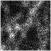
\includegraphics[width=0.2\textwidth]{blinking-1-8a.png}}
		\hfill
		\subcaptionbox{Усреднённое по времени изображение}[0.3\textwidth]{%
			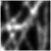
\includegraphics[width=0.2\textwidth]{blinking-1-8b.png}}
		\hfill
		\subcaptionbox{Результат обработки серии изображений}[0.3\textwidth]{%
			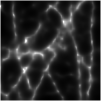
\includegraphics[width=0.2\textwidth]{blinking-1-8h.png}}
		\hfill
	}
	\caption{Результат обработки реальной серии снимков предложенным методом}
	\label{fig:sinopsis-blinking}
\end{figure}

Сравнение с рядом существующих алгоритмов показало, что разработанный метод позволяет восстанавливать резкое изображение, его достоинством являются имеющие физический смысл восстановленные яркость и дисперсия яркости точек изображения.
%, а недостатком "--- высокая вычислительная сложность.


%TODO Глава 2
Во {\textbf{второй}} главе рассматривается задача повышения резкости медицинских изображений методом деформации пиксельной сетки. Проводится поиск оптимальной функции смещения пикселей для этого метода для каждого модельных ядер размытия.

Используемая модель размытия изображения представляет собой свёртку резкого изображения с ядром размытия. Рассматриваются три модели реалистичных ядер оптического размытия с параметрами $\sigma$ и $r$:
\begin{enumerate}[beginpenalty=10000]
	\item Гауссово ядро.
	Задаётся формулой
	$$f_\sigma\left(x,y\right) = \frac{1}{2\pi\sigma^2}\exp\left(-\frac{x^2+y^2}{2\sigma^2}\right).$$
	%	Радиусом этого ядра будет считаться величина $3\sigma$.
	%	Радиусом этого ядра будет считаться величина $1.5\sigma$.
	
	\item Ядро типа <<круг>>.
	Задаётся формулой $$f_r\left(x,y\right) = \begin{cases}
		1, & x^2 + y^2 \leq r^2, \\
		0, & \text{иначе}.
	\end{cases}$$
	%	Радиус ядра "--- радиус круга $r$.
	
	\item Ядро типа <<круг с кольцом>>.
	Задаётся формулой $$f_r(x, y) = \begin{cases}
		0.25, & x^2 + y^2 \leq 0.75 r^2,\\
		1, & 0.75 r^2 < x^2 + y^2 \leq r^2,\\
		0, & \text{иначе}.
	\end{cases}$$
	%	Радиус ядра "--- радиус круга $r$.
\end{enumerate}

\noindent Примеры таких ядер представлены на Рис.~\ref{fig:sinopsis-warping-blur}.

\begin{figure}[ht]
	\centerfloat{
		\hfill
		\subcaptionbox[List-of-Figures entry]{Гауссово ядро (Г)}{%
			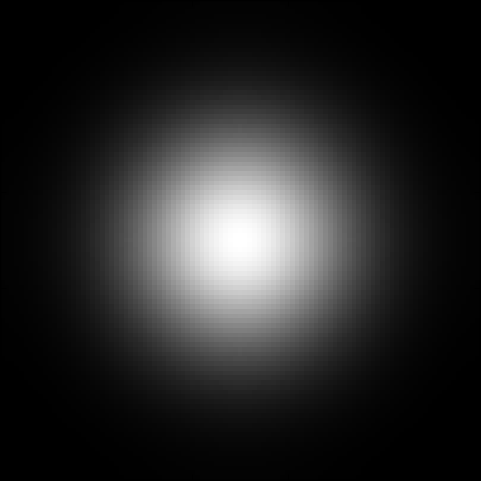
\includegraphics[width=0.25\textwidth]{warping-1-3a.png}}
		\hfill
		\subcaptionbox{Круг (К)}{%
			
\includegraphics[width=0.25\textwidth]{warping-1-3b.png}}
		\hfill
		\subcaptionbox{Круг с кольцом (КЦ)}{%
			
\includegraphics[width=0.25\textwidth]{warping-1-3c.png}}
		\hfill
	}
	\caption{Рассматриваемые во второй главе модели ядер размытия}
	\label{fig:sinopsis-warping-blur}
\end{figure}

В процессе работы алгоритма:
\begin{enumerate}[beginpenalty=10000]
	\item на изображении обнаруживаются контуры,
	\item оценивается значение параметра размытия,
	\item производится вычисление векторов смещения пикселей в окрестности обнаруженных контуров по направлению к этим контурам,
	\item в соответствии с вычисленным векторным полем смещений деформируется пиксельная сетка,
	\item полученный результат проецируется на равномерную сетку выходного изображения с помощью интерполяции.
\end{enumerate}

В работе двумерное поле смещений $\vec{d}\left(x,y\right)$ вычисляется через одномерную функцию смещения $d\left(x\right)$ с учётом расстояния пикселя до ближайших контуров и величины градиента на этих контурах:

\begin{equation*}
	\vec{d}\left(x,y\right) = \frac{\sum_{\left(x_e,y_e\right) \in N\left(x,y\right)}{d\left(x_n\right) G_{\widetilde{\sigma}}\left(x_t\right) \vec{g}\left(x_e,y_e\right) }} {\sum_{\left(x_e,y_e\right) \in N\left(x,y\right)}{G_{\widetilde{\sigma}}\left(x_t\right)\lvert \vec{g}\left(x_e,y_e\right) \rvert}}.
\end{equation*}

\noindent где $N\left(x,y\right)$ "--- это множество точек контуров в окрестности т.~$\left(x, y\right)$; $x_n$ и $x_t$ "--- это проекции вектора $\left(x-x_e, y-y_e\right)$ на вектор градиента изображения $\vec{g}\left(x_e,y_e\right)$ и на нормаль к нему соответственно. Весовая функция $G_{\widetilde{\sigma}}\left(x_t\right)$ определяется формулой:

\begin{equation*}
	G_{\widetilde{\sigma}}\left(x\right) = \frac{1}{\widetilde{\sigma} \sqrt{2\pi}} \exp\left(\frac{-x^2}{2\widetilde{\sigma}^2}\right),
\end{equation*}

\noindent где $\widetilde{\sigma}$ "--- настраиваемый параметр, для которого в ходе выполнения исследования использовалось значение, равное $2.5$ параметрам размытия. В качестве основы выступает одномерная функция смещения $d\left(x_n\right)$.

В работе предлагаются две новые модели функции смещения:

\begin{enumerate}[beginpenalty=10000]	
	\item
	$
	\begin{aligned}
		d_2\left(x; a, b, c\right)=\left\{
		\begin{aligned}
			&\frac{c}{a}x,\ \left|x\right|<a,\\
			&c\frac{b-\left|x\right|}{b-a} \cdot sign\left(x\right),\ a\le\left|x\right|<b,\\
			&0,\ \left|x\right|\geq b;
		\end{aligned}
		\right.
	\end{aligned}
	$
	
	\item $d_1\left(x; a, c\right) = d_2\left(x; a, 1.5a, c\right)$,
\end{enumerate}

\noindent а также рассмотрена и использована для оценки повышения эффективности алгоритма модель функции смещения, соответствующая функции близости, предложенной в статье авторов деформационного метода:

$d_0\left(x; s\right)=s\sqrt\pi\left[erf\left(\frac{x}{2s}\right)-erf\left(\frac{x}{s}\right)\right]$, где $erf{\left(x\right)}=\frac{2}{\sqrt\pi}\int_{0}^{x}{e^{-t^2}dt}$.

При этом величина $x$ "--- это расстояние от точки до контура, делённое на параметр ядра размытия, что позволяет масштабировать функцию для разных уровней размытия без изменения самих параметров $a$, $b$, $c$ и $s$.

Поиск оптимальных параметров для каждого ядра размытия проводится путём минимизации показателя RMSE по всем изображениях тестового набора, состоящего из 192 изображений, созданных путём размытия с разной силой естественных изображений из базы TID2013.

Эксперименты показали, что предложенные функции смещения $d_2\left(x\right)$ и $d_1\left(x\right)$ демонстрируют улучшение качества обработки изображений по сравнению с оригинальной функцией $d_0\left(x\right)$, выражаемое в приросте показателя PNSR (см.~Табл.~\ref{tab:synopsis-warping-psnr}).
%, в среднем на 27\%. 
Вариант алгоритма на основе однопараметрической функция смещения $d_1\left(x\right)$ почти не отличается от двухпараметрического варианта качеством результатов (там же), благодаря этому можно использовать его для всех трёх рассмотренных ядер размытия.

\begin{table} [htbp]%
	\centering
	\caption{Средние значения показателя качества PSNR по всем уровням размытия}%
	\label{tab:synopsis-warping-psnr}% label всегда желательно идти после caption
	\renewcommand{\arraystretch}{1.5}%% Увеличение расстояния между рядами, для улучшения восприятия.
	\begin{SingleSpace}
		\begin{tabulary}{\textwidth}{@{}@{\extracolsep{10pt}}lCCCC@{}} %Вертикальные полосы не используются принципиально, как и лишние горизонтальные (допускается по ГОСТ 2.105 пункт 4.4.5) % @{} позволяет прижиматься к краям
			\toprule     %%% верхняя линейка
			Ядро & Размытое изображение & $d_0\left(x\right)$ & $d_2\left(x\right)$ & $d_1\left(x\right)$ \\
			\midrule %%% тонкий разделитель. Отделяет названия столбцов. Обязателен по ГОСТ 2.105 пункт 4.4.5
			Гауссово & 23.104 & 23.361 & 23.419 & 23.419 \\
			Круг & 24.825 & 25.053 & 25.110 & 25.110 \\
			Круг с кольцом & 24.005 & 24.252 & 24.351 & 24.346 \\
			\bottomrule %%% нижняя линейка
		\end{tabulary}%
	\end{SingleSpace}
\end{table}

Дополнительный анализ показал, что при несильном отклонении параметра от оптимального значения качество результирующего изображения снижается слабо (см. Рис.~\ref{fig:synopsis-warping-isnr-change}).

\begin{figure}[ht]
	\centerfloat{
		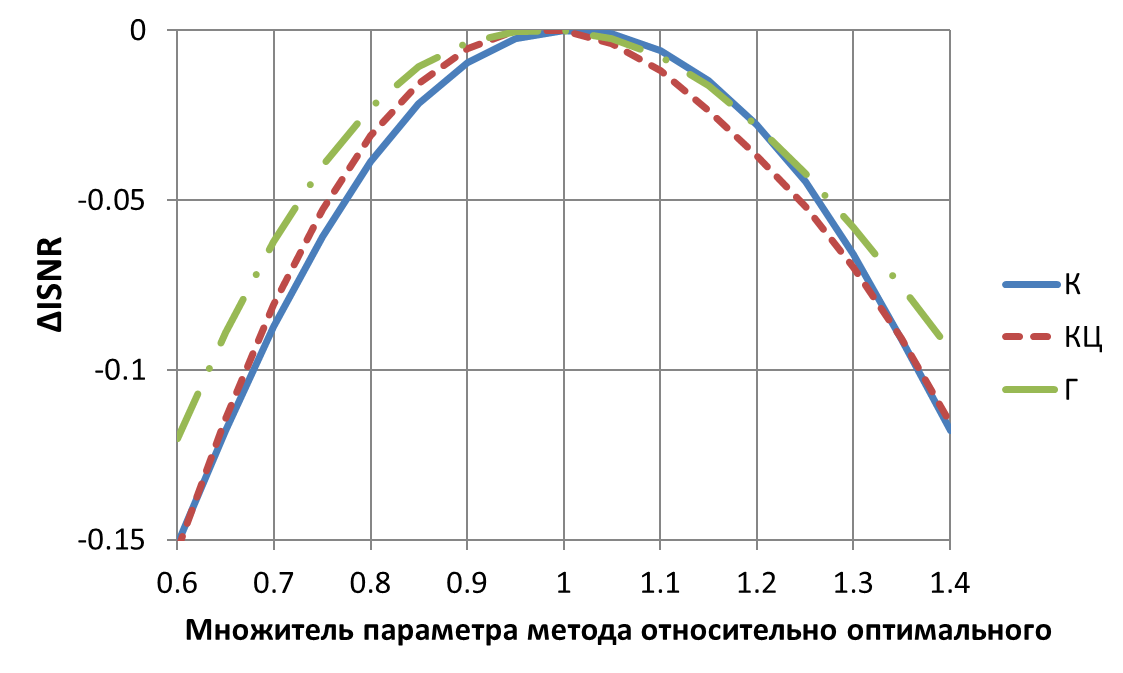
\includegraphics[width=0.8\textwidth]{warping-1-extra1-gray.png}
	}
	\caption{Изменение ISNR (прироста показателя PSNR) при относительном изменении параметра $a$}
	\label{fig:synopsis-warping-isnr-change}
\end{figure}


%TODO Глава 3
В {\textbf{третьей}} главе исследуется вопрос контроля качества изображений в задаче компьютерной диагностики туберкулёза. Рассматриваются:
\begin{enumerate}[beginpenalty=10000]
	\item задача автоматического определения уровня жёсткости рентгеновского снимка грудной клетки с помощью нейросетевого алгоритма;
	\item влияние предварительной фильтрации обучающей и валидационной выборок на качество работы алгоритма классификации в задаче диагностики туберкулёза лёгких по рентгеновским снимкам грудной клетки.
\end{enumerate}

При изучении рентгеновских снимков грудной клетки, и в частности при диагностике туберкулёза лёгких, важным фактором является жёсткость снимка, так как она напрямую влияет на его информативность.
%~\cite{chuiko1982effects, тимофеева2013основные}. 
Уровень жёсткости обусловлен дозой радиации, длиной волны излучения и особенностями тела пациента. При условии правильного контрастирования снимка уровень жёсткости можно определить визуально, подсчитав число отчётливо видимых на снимке верхних грудных позвонков: оптимальному уровню в задаче диагностики туберкулёза лёгких соответствуют 3"~4 видимых позвонка, а меньшее или большее число свидетельствует о том, что снимок слишком мягкий или жёсткий.
%~\cite{тимофеева2013основные, сидоров2012методика}. 
Пример рентгеновского изображения позвоночного столба с указанием номеров позвонков приведён на Рис.~\ref{fig:synopsis-vertebral-column}, а примеры снимков разного уровня жёсткости представлены на Рис.~\ref{fig:synopsis-samples-different-hardness}.

\begin{figure}[ht]
	\centerfloat{
		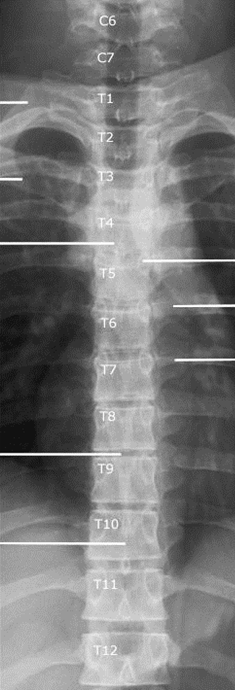
\includegraphics[height=0.3\textheight]{example_vertebrae.png}
	}
	\caption{Пример рентгеновского изображения позвоночника с номерами шейных (C) и грудных (T) позвонков}
	\label{fig:synopsis-vertebral-column}
\end{figure}

\begin{figure}[ht]
	\centerfloat{
		\hfill
		\subcaptionbox[List-of-Figures entry]{Мягкий снимок}{%
			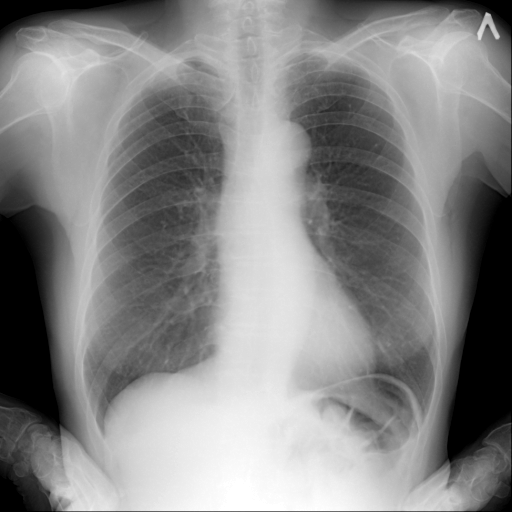
\includegraphics[width=0.3\textwidth]{example_soft.png}}
		\hfill
		\subcaptionbox{Нормальный снимок}{%
			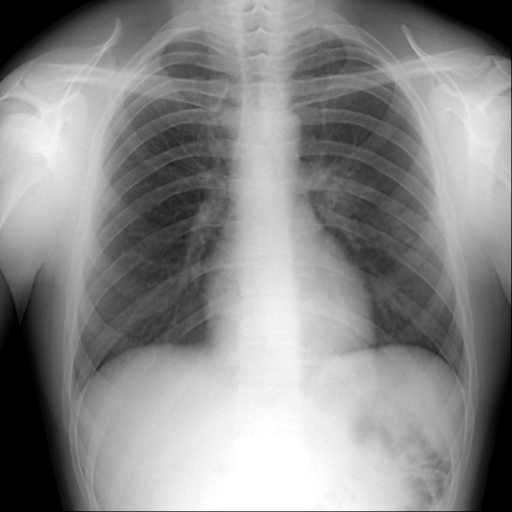
\includegraphics[width=0.3\textwidth]{example_normal.png}}
		\hfill
		\subcaptionbox{Жёсткий снимок}{%
			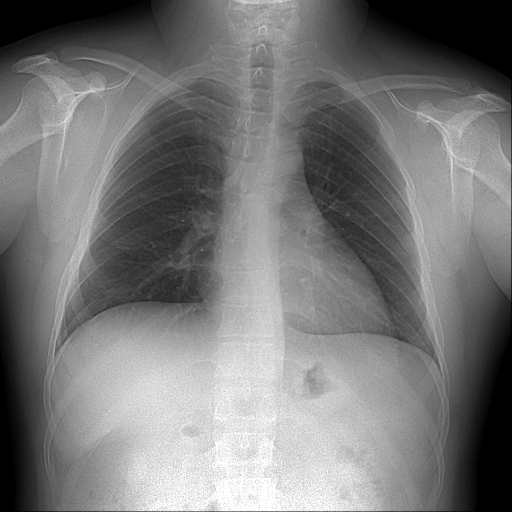
\includegraphics[width=0.3\textwidth]{example_hard.png}}
		\hfill
	}
	\caption{Примеры рентгеновских снимков грудной клетки разной жёсткости}
	\label{fig:synopsis-samples-different-hardness}
\end{figure}

В ходе выполнения работы разработан метод автоматического анализа качества рентгенограмм грудной клетки, основанный на нейросетевой оценке уровня жёсткости рентгеновских снимков. Процесс обучения его нейросетевой модели выглядит следующим образом:
\begin{enumerate}[beginpenalty=10000]
	\item предобработка входных данных;
	\item итерационный процесс минимизации функции потерь (функционала, отображающего выходные значения нейросетевой модели в показатель их близости к оптимальным значениям для решения задачи) повторением шагов:
	\begin{enumerate}[beginpenalty=10000]
		\item подача предобработанных выходных данных на вход нейросетевой модели и получение её выходных значений;
		\item получение значения функции потерь для данных выходных значений модели и входных данных;
		\item шаг оптимизации;
		\item замер качества работы алгоритма;
		\item проверка условия ранней остановки процесса минимизации;
	\end{enumerate}
	\item сохранение модели.	
\end{enumerate}

Процесс применения метода состоит из следующих шагов:
\begin{enumerate}[beginpenalty=10000]
	\item предобработка входных данных;
	\item подача предобработанных выходных данных на вход нейросетевой модели и получение её выходных значений;
\end{enumerate}

При решении задачи были использованы два набора рентгенограмм грудной клетки, снятых во фронтальной проекции: собранный в сотрудничестве с медиками из НПЦ~<<Фтизиатрия>> им. Е.Н.~Андреева в г. Якутске набор применялся для обучения нейросетевой модели для метода определения жёсткости рентгенограмм; набор, сформированный из двух наиболее часто используемых при разработке методов компьютерной диагностики туберкулёза лёгких общедоступных наборов рентгенограмм, применялся для оценки качества работы разработанного алгоритма на снимках, сделанных в других медицинских учреждениях, на другом оборудовании и при других условиях. Аннотирование обоих использованных наборов проводилось врачом-рентгенологом из НПЦ~<<Фтизиатрия>> им. Е.Н.~Андреева, каждому изображению ставился в соответствие его уровень жёсткости, выраженный числом отчётливо видимых на этом снимке верхних грудных позвонков. Для снижения несбалансированности обучающего набора все снимки были разделены по уровню жёсткости на 3 группы согласно медицинским критериям: мягкие (видно менее 3 позвонков), нормальные (видно 3"~4 позвонка) и жёсткие (видно более 4 позвонков), получившееся соотношение классов представлено на Рис.~\ref{fig:synopsis-hardness-yak-hardness}.

\begin{figure}[ht]
	\centerfloat{
		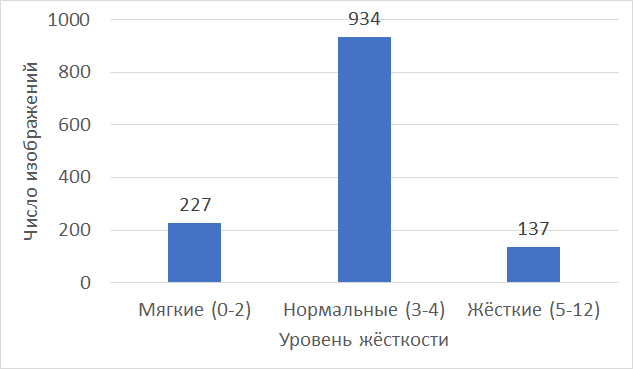
\includegraphics[height=0.25\textheight]{total_hardness_hist.png}
	}
	\caption{Гистограмма распределения снимков набора Sakha"~TB* по уровню жёсткости}
	\label{fig:synopsis-hardness-yak-hardness}
\end{figure}

Хотя финальным критерием при определении уровня жёсткости рентгеновского снимка грудной клетки является число чётко контурируемых верхних грудных позвонков,
%~\cite{тимофеева2013основные, сидоров2012методика}, 
для определения уровня контрастности перед исследованием требуется обращать внимание на видимость других областей грудной клетки (например, на элементы лёгочного рисунка) и органов.
%~\cite{сидоров2012методика}. 
На основании этого было принято решение не ограничивать область исследования на снимках пределами грудной клетки, а рассматривать изображения целиком.

Так как условия получения снимка, характеристики тела пациента и принципы считывания сигнала и хранения информации каждого конкретного устройства могут сильно влиять на характер рентгеновских изображений, перед подачей их на вход алгоритма определения жёсткости необходим этап предобработки. В ходе выполнения исследования был разработан алгоритм адаптивного контрастирования, который заключается в последовательности следующих шагов:
\begin{enumerate}[beginpenalty=10000]
	\item автоматическое контрастирование изображения:
	\begin{equation}
		h \left( x \right) = 255 \cdot \frac{x - p_{0.5}}{p_{99.5} - p_{0.5}}, \nonumber
	\end{equation}
	где $x$ "--- значение интенсивности пикселя входного изображения, $p_{0.5}$ и $p_{99.5}$ "--- это 0.5\%"~ и 99.5\%"~процентили значений интенсивности всех пикселей изображения;
	\item автоматическая гамма-коррекция интенсивности пикселей изображения:
	\begin{equation}
		g \left( x \right) = 255 \cdot {\left( \frac{x}{255} \right)}^{\gamma}, \quad \gamma = \log_{\mu / 255}{0.5}, \nonumber
	\end{equation}
	где $\mu$ "--- средняя интенсивность всего изображения;
	\item уменьшение изображения до входного разрешения, используемого нейронной сетью, при помощи билинейной интерполяции;
%	 (512х512 пикселей для модели на основе ResNet"~18 и 384x384 пикселей для модели на основе EfficientNetV2"~S).
	\item опциональный шаг глобальной или локальной (CLAHE) эквализации гистограммы. Размер стороны квадратного окна  в пикселях, использованного в методе локальной эквализации гистограммы, прямо зависел от размера стороны изображения и составлял $\frac{1}{2^n}$ от него, где $n\in\mathbb{N}$ "--- параметр метода.
%	Влияние наличия этого шага и размера окна на качество работы алгоритма будет показано ниже.
\end{enumerate}

\noindent Примеры результатов работы разработанного алгоритма адаптивного контрастирования с разными параметрами шага 4 представлены на Рис.~\ref{fig:synopsis-preprocessing-examples}.

\begin{figure}[ht]
	\centerfloat{
		%		\hfill
		\subcaptionbox[List-of-Figures entry]{Исходные изображения}{%
			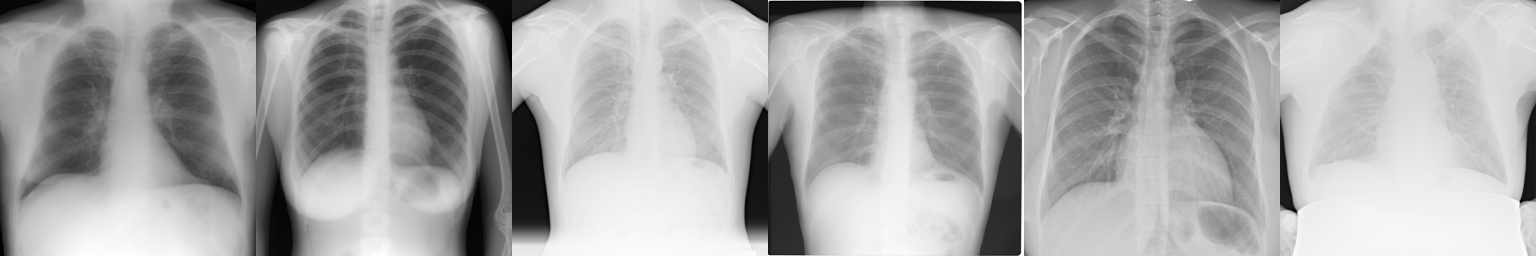
\includegraphics[width=0.9\linewidth]{preprocessing-before.png}}
		%		\hfill
		\vfill
		%		\hfill
		\subcaptionbox{Предобработка без эквализации гистограммы}{%
			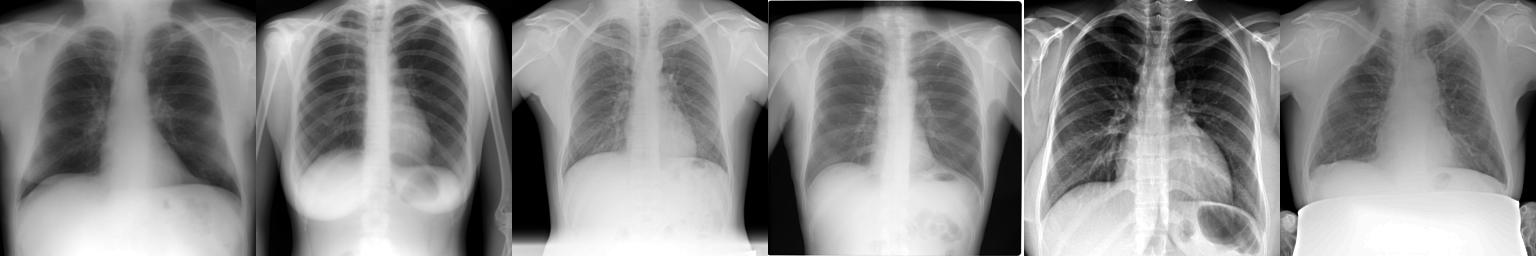
\includegraphics[width=0.9\linewidth]{preprocessing-noequalize.png}}
		%		\hfill
		\vfill
		%		\hfill
		\subcaptionbox{Предобработка с глобальной эквализацией гистограммы}{%
			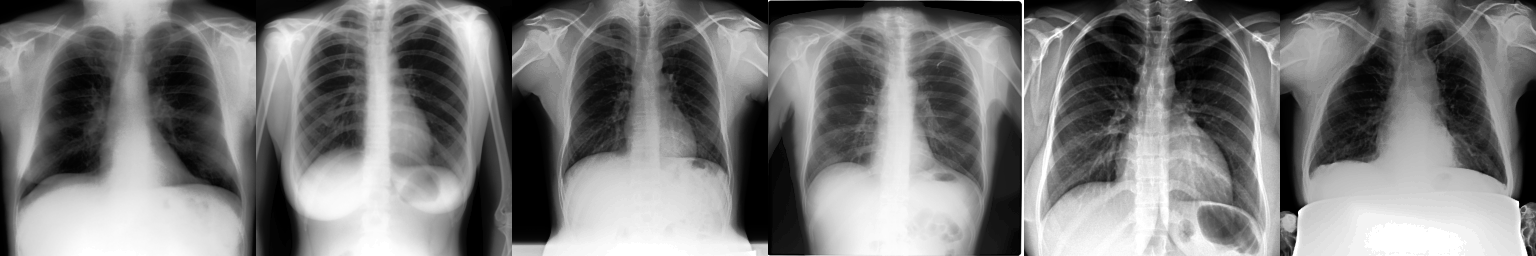
\includegraphics[width=0.9\linewidth]{preprocessing-global.png}}
		%		\hfill
		\vfill
		%		\hfill
		\subcaptionbox{Предобработка с локальной эквализацией гистограммы, $n=1$}{%
			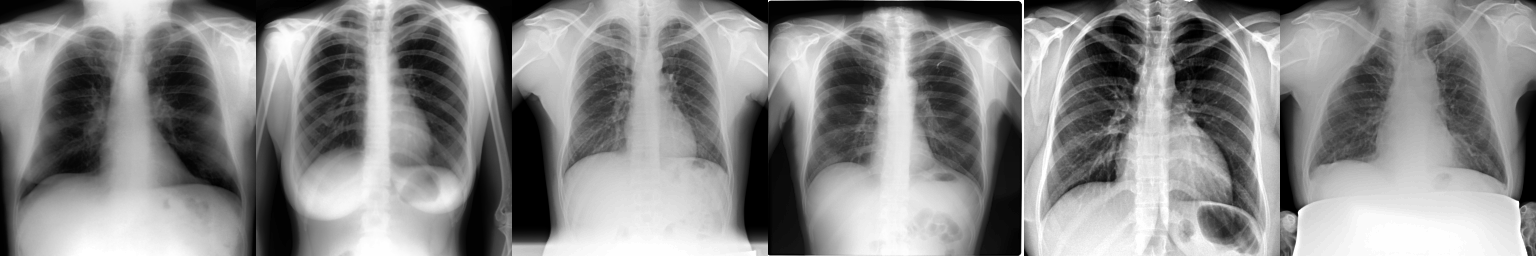
\includegraphics[width=0.9\linewidth]{preprocessing-clahe-2.png}}
		%		\hfill
		\vfill
		%		\hfill
		\subcaptionbox{Предобработка с локальной эквализацией гистограммы, $n=3$}{%
			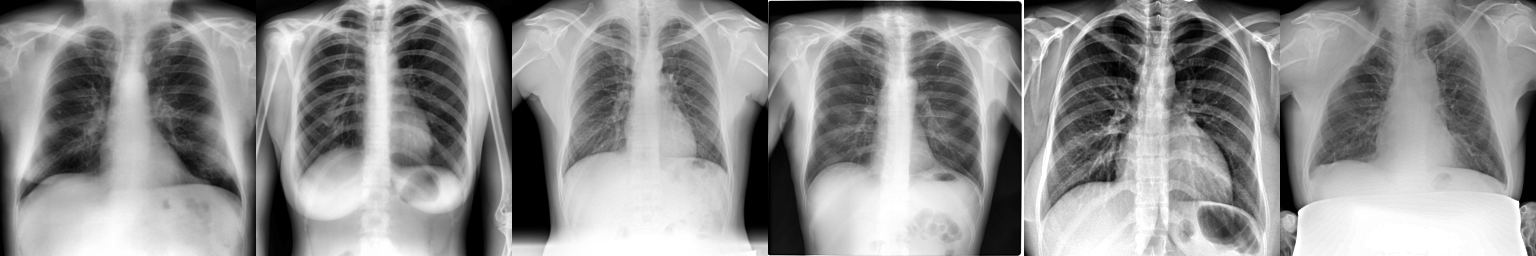
\includegraphics[width=0.9\linewidth]{preprocessing-clahe-8.png}}
		%		\hfill
		\vfill
	}
	\caption{Примеры результатов предварительной обработки рентгенограмм}
	\label{fig:synopsis-preprocessing-examples}
\end{figure}

Для сохранения отношений упорядоченности между классами задача определения уровня жёсткости рентгеновского снимка рассматривалась как задача порядковой регрессии. Последний слой нейронной сети был заменён на полносвязный слой с 1 выходом и 2 настраиваемыми в процессе обучения параметрами"=порогами пороговой модели порядковой регрессии, во время дальнейшего обучения были задействованы все слои. На вход разработанного алгоритма поступает рентгеновский снимок грудной клетки и подвергается предобработке, затем при помощи нейронной сети ему ставится в соответствие вещественное число на отрезке $\left[0, 1\right]$, которое является внутренним безразмерным показателем жёсткости снимка, на основании которого после сравнения с настраиваемыми порогами изображение относится к одному из рассматриваемых классов жёсткости. Преимуществом такого подхода является то, что с помощью внутреннего показателя жёсткости можно ранжировать изображения относительно друг друга даже в том случае, когда обрабатываемое изображение значительно отличается от обучающей выборки и для такого снимка пороги разделения классов жёсткости могут быть настроены неверно.

Применялась свёрточные нейронные сети на основе архитектуры ResNet"~18 
%~\cite{he2016deep} 
со входным разрешением 512х512 пикселей и на основе EfficientNetV2"~S 
%~\cite{tan2021efficientnetv2} 
со входным разрешением 384x384 пикселя. Последний слой нейронных сетей был заменён на полносвязный слой с 1 выходом и 2 настраиваемыми в процессе обучения параметрами"=порогами пороговой модели порядковой регрессии,
%~\cite{rennie2005loss}, 
во время дальнейшего обучения были задействованы все слои.

Набор рентгенограмм, использованный для обучения алгоритма, делился на обучающую, валидационную и тестовую выборку. Изображения обучающей выборки в процессе обучения подвергались случайным преобразованиям. Применялось взвешивание значений функции потерь для каждого примера обучающей выборки с весами, обратно пропорциональными количеству изображений соответствующего класса.

В качестве функции потерь в процессе обучения и валидации была выбрана функция потерь пороговой порядковой регрессии в виде суммы слагаемых, число которых зависит от числа классов (all"=threshold):
%~\cite{rennie2005loss}:

\begin{equation}
	\begin{cases}
		L \left( z, y, \theta_1, \ldots, \theta_{K-1} \right) = \sum_{k=1}^{K-1} f \left( s \left( k, y \right) \cdot \left( \theta_k-z \right) \right), \\
		s \left( k, y \right) =
		\begin{cases}
			-1, k < y, \\
			+1, \ k \geq y,
		\end{cases}
	\end{cases} \nonumber
\end{equation}

\noindent где $z$ "--- выход нейронной сети (безразмерный показатель жёсткости), принимающий значения из отрезка $\left[ 0, 1 \right]$ (чем ближе к $1$, тем выше жёсткость снимка), $y$ "--- истинный класс соответствующего этому выходу изображения, $K$ "--- общее число классов (в ходе выполнения работы равное 3), $\theta_1 < \theta_2 < \ldots < \theta_{K-1}$ "--- пороги, делящие действительную прямую на $K$ частей, а $f(x)$ "--- базовая функция потерь бинарной классификации, в качестве которой использовалась логистическая функция потерь:

\begin{equation}
	f \left( x \right) = \ln{\frac{1}{1+e^{-x}}}. \nonumber
\end{equation}

Результаты оценки жёсткости рентгенограмм были использованы для предварительной фильтрации обучающей выборки и входных данных нейросетевого алгоритма компьютерной диагностики туберкулёза лёгких по рентгеновским снимкам грудной клетки. Для создания и тестирования методов диагностики применялись три широко используемых общедоступных наборов рентгенограмм грудной клетки здоровых и больных туберкулёзом лёгких пациентов: Montgomery County, 
%~\cite{candemir2013lung}, 
Shenzhen 
%~\cite{jaeger2013automatic} 
и TBX11K.
%~\cite{liu2020rethinking}.

На основании предсказанных величин жёсткости было проведено удаление из объединённого набора изображений одинаковой доли самых жёстких и самых мягких снимков (то есть с обеих сторон гистограммы распределения величин жёсткости). После этого качество обученного на прореженной обучающей выборке метода диагностики замерялось на прореженной тестовой выборке и сравнивалось с качеством работы на такой же тестовой выборке модели диагностики, обученной на непрореженной обучающей выборке.

Помимо прореживания выборок с обеих сторон гистограммы уровня жёсткости был рассмотрен и случай отбрасывания только самых жёстких снимков, так как на мягких снимках ещё могут сохраняться некоторые детали лёгочной ткани, в то время как на жёстких они могут быть полностью утеряны.

Значения сбалансированной точности, полученные в результате экспериментов представлены в Табл.~\ref{tab:synopsis-hardness-filtering-balacc}. Из неё видно, что изменение качества зависит от степени прореживания изображений, однако остаётся стабильно положительным. Сравнение более распространённых в медицине показателей чувствительности и специфичности для класса больных туберкулёзом пациентов приведено в Табл.~\ref{tab:synopsis-hardness-filtering-sens-spec}.

\begin{table} [htbp]%
	\centering
	\caption{Сравнение качества классификации моделей, обученных на полном и прореженном наборе (сбалансированная точность)}%
	\label{tab:synopsis-hardness-filtering-balacc}% label всегда желательно идти после caption
	\renewcommand{\arraystretch}{1.5}%% Увеличение расстояния между рядами, для улучшения восприятия.
	\begin{SingleSpace}
		\begin{tabulary}{\textwidth}{@{}@{\extracolsep{10pt}}cCCCCCC@{}} %Вертикальные полосы не используются принципиально, как и лишние горизонтальные (допускается по ГОСТ 2.105 пункт 4.4.5) % @{} позволяет прижиматься к краям
			\toprule     %%% верхняя линейка
			& \multicolumn{3}{@{}c@{}}{\makecell{Удаление жёстких и \\ мягких изображений}} & \multicolumn{3}{@{}c@{}}{\makecell{Удаление только \\ жёстких изображений}} \\
			\cmidrule(r){2-4}\cmidrule(l){5-7}
			Доля удалённых & 5\% & 10\% & 15\% & 5\% & 10\% & 15\% \\
			\midrule %%% тонкий разделитель. Отделяет названия столбцов. Обязателен по ГОСТ 2.105 пункт 4.4.5
			До прореживания& 0.958 & 0.951 & 0.951 & 0.962 & 0.961 & 0.965 \\
			После прореживания& 0.961 & 0.962 & 0.953 & 0.968 & 0.966 & 0.975 \\
			\bottomrule %%% нижняя линейка
		\end{tabulary}%
	\end{SingleSpace}
\end{table}

\begin{table} [htbp]%
	\centering
	\caption{Сравнение качества классификации моделей, обученных на полном и прореженном наборе (чувствительность~/~специфичность)}%
	\label{tab:synopsis-hardness-filtering-sens-spec}% label всегда желательно идти после caption
	\renewcommand{\arraystretch}{1.5}%% Увеличение расстояния между рядами, для улучшения восприятия.
	\begin{SingleSpace}
		\begin{tabulary}{\textwidth}{@{}@{\extracolsep{10pt}}cCCCCCC@{}} %Вертикальные полосы не используются принципиально, как и лишние горизонтальные (допускается по ГОСТ 2.105 пункт 4.4.5) % @{} позволяет прижиматься к краям
			\toprule     %%% верхняя линейка
			& \multicolumn{3}{@{}c@{}}{\makecell{Удаление жёстких и \\ мягких изображений}} & \multicolumn{3}{@{}c@{}}{\makecell{Удаление только \\ жёстких изображений}} \\
			\cmidrule(r){2-4}\cmidrule(l){5-7}
			Доля удалённых & 5\% & 10\% & 15\% & 5\% & 10\% & 15\% \\
			\midrule %%% тонкий разделитель. Отделяет названия столбцов. Обязателен по ГОСТ 2.105 пункт 4.4.5
			До прореживания& 0.923/ 0.994 & 0.909/ 0.994 & 0.908/ 0.995 & 0.930/ 0.994 & 0.927/ 0.995 & 0.934/ 0.996 \\
			После прореживания& 0.933/ 0.990 & 0.933/ 0.991 & 0.915/ 0.990 & 0.943/ 0.994 & 0.941/ 0.992 & 0.958/ 0.993 \\
			\bottomrule %%% нижняя линейка
		\end{tabulary}%
	\end{SingleSpace}
\end{table}

Разработанный метод определения жёсткости позволяет увеличить качество работы алгоритма диагностики туберкулёза лёгких при условии предварительной фильтрации изображений перед обучением классификатора и получением предсказаний. Снижение разброса жёсткости данных и увеличение их однородности заметно повысило точность обнаружения больных пациентов при сохранении или малом снижении специфичности.


%TODO Глава 4
{\textbf{Четвёртая}} глава посвящена программной реализации алгоритмов, разработанных в предыдущих главах. Описывается разработанный программный комплекс, состоящий из трёх различных программных модулей:
\begin{enumerate}[beginpenalty=10000]
	\item модуль повышения разрешения изображений мигающей флуоресцентной микроскопии;
	
	\item модуль повышения резкости медицинских изображений методом деформации пиксельной сетки;
	
	\item модуль анализа и обработки рентгенограмм грудной клетки.
\end{enumerate}

Представлено описание интерфейса программных модулей. Программная реализация модулей выполнялась на языке программирования Python~3 с применением программных библиотек для работы с математическими функциями и векторными вычислениями и для машинного обучения.

Кроме того, приводится описание сформированного в ходе выполнения работы набора рентгенограмм грудной клетки для задачи компьютерной диагностики туберкулёза и демонстрируется возможность повысить с его помощью качество диагностики для некоторых нейросетевых алгоритмов.


%TODO: Заключение
\FloatBarrier
\pdfbookmark{Заключение}{conclusion}                                  % Закладка pdf
В \textbf{заключении} формулируются основные результаты работы, которые заключаются в следующем:
%% Согласно ГОСТ Р 7.0.11-2011:
%% 5.3.3 В заключении диссертации излагают итоги выполненного исследования, рекомендации, перспективы дальнейшей разработки темы.
%% 9.2.3 В заключении автореферата диссертации излагают итоги данного исследования, рекомендации и перспективы дальнейшей разработки темы.
\begin {enumerate}
	\item Разработан итерационный регуляризирующий алгоритм повышения разрешения и резкости изображений флуоресцентной мигающей микроскопии.
	\item Найдены оптимальные функции смещения для деформационного метода повышения резкости изображений для трёх видов ядер размытия, возникающих на практике. Предложен однопараметрический вариант алгоритма.
	\item Разработан нейросетевой метод контроля качества рентгеновских снимков грудной клетки, основанный на визуальном определении жёсткости рентгенограммы. Показана возможность повышения качества диагностики с его помощью.
	\item TODO: Этой главы пока нету. - Реализован программный комплекс, состоящий из модулей повышения разрешения изображений флуоресцентной мигающей микроскопии, повышения резкости медицинских изображений, определения качества рентгенограмм грудной клетки для задачи диагностики туберкулёза и компьютерной диагностики туберкулёза.
\end {enumerate}



\pdfbookmark{Литература}{bibliography}                                % Закладка pdf

\ifdefmacro{\microtypesetup}{\microtypesetup{protrusion=false}}{} % не рекомендуется применять пакет микротипографики к автоматически генерируемому списку литературы
\urlstyle{rm}                               % ссылки URL обычным шрифтом
\ifnumequal{\value{bibliosel}}{0}{% Встроенная реализация с загрузкой файла через движок bibtex8
    \renewcommand{\bibname}{\large \bibtitleauthor}
    \nocite{*}
    \insertbiblioauthor           % Подключаем Bib-базы
    %\insertbiblioexternal   % !!! bibtex не умеет работать с несколькими библиографиями !!!
}{% Реализация пакетом biblatex через движок biber
    % Цитирования.
    %  * Порядок перечисления определяет порядок в библиографии (только внутри подраздела, если `\insertbiblioauthorgrouped`).
    %  * Если не соблюдать порядок "как для \printbibliography", нумерация в `\insertbiblioauthor` будет кривой.
    %  * Если цитировать каждый источник отдельной командой --- найти некоторые ошибки будет проще.
    %
    %% authorvak
%    \nocite{vakbib1}%
%    \nocite{vakbib2}%
    %
    %% authorwos
%    \nocite{wosbib1}%
    %
    %% authorscopus
%    \nocite{scbib1}%
    %
    %% authorpathent
%    \nocite{patbib1}%
    %
    %% authorprogram
%    \nocite{progbib1}%
    %
    %% authorconf
%    \nocite{confbib1}%
%    \nocite{confbib2}%
    %
    %% authorother
%    \nocite{bib1}%
%    \nocite{bib2}%
    
	\nocite{krylov2017single}
	\nocite{krylov2018grid171613482}
	\nocite{krylovpost}
	\nocite{pchelintsev2019enhancement}
	\nocite{krylov2021regularization386034310}
	\nocite{dovganich2022automatic}
	\nocite{pchelintsev2023hardness}
	\nocite{pchelintsev2023robustness}

    \ifnumgreater{\value{usefootcite}}{0}{
        \begin{refcontext}[labelprefix={}]
            \ifnum \value{bibgrouped}>0
                \insertbiblioauthorgrouped    % Вывод всех работ автора, сгруппированных по источникам
            \else
                \insertbiblioauthor      % Вывод всех работ автора
            \fi
        \end{refcontext}
    }{
        \ifnum \totvalue{citeexternal}>0
            \begin{refcontext}[labelprefix=A]
                \ifnum \value{bibgrouped}>0
                    \insertbiblioauthorgrouped    % Вывод всех работ автора, сгруппированных по источникам
                \else
                    \insertbiblioauthor      % Вывод всех работ автора
                \fi
            \end{refcontext}
        \else
            \ifnum \value{bibgrouped}>0
                \insertbiblioauthorgrouped    % Вывод всех работ автора, сгруппированных по источникам
            \else
                \insertbiblioauthor      % Вывод всех работ автора
            \fi
        \fi
        %  \insertbiblioauthorimportant  % Вывод наиболее значимых работ автора (определяется в файле characteristic во второй section)
        \begin{refcontext}[labelprefix={}]
            \insertbiblioexternal            % Вывод списка литературы, на которую ссылались в тексте автореферата
        \end{refcontext}
        % Невидимый библиографический список для подсчёта количества внешних публикаций
        % Используется, чтобы убрать приставку "А" у работ автора, если в автореферате нет
        % цитирований внешних источников.
        \printbibliography[heading=nobibheading, section=0, env=countexternal, keyword=biblioexternal, resetnumbers=true]%
    }
}
\ifdefmacro{\microtypesetup}{\microtypesetup{protrusion=true}}{}
\urlstyle{tt}                               % возвращаем установки шрифта ссылок URL
